\begin{exercise}{5.6}
    Consider the eigenvalues of the operators, $L_1$, $L_2$, and $L_3$, where $L_1 u = u_x$, $L_2 u = -\alpha u_{xx}$, $\alpha = 1.0 e^{-5}$, and $L_3 = L_1 + L_2$, with homogeneous Dirichlet conditions.
    For which of the operators are the eigenvalues positive and real?
    Repeat the exercise with $L_1 = x u_x$.
\end{exercise}

\begin{solution}{5.6}
    Here, I assume that the domain is $[0, 1]$, and the boundary conditions are $u(0) = u(1) = 0$.
    Solving for the eigenvalues for the first operators is not terribly difficult, although it is a bit tedious.
    Instead, we will use the finite element method.

    With the eigenvalue problem $L u = \lambda u$, we have the associated weak form
    \begin{equation*}
        \int_0^1 L u \, v \, \diff x = \lambda \int_0^1 u \, v \, \diff x,
    \end{equation*}
    where $L$ is one of the operators $L_1$, $L_2$, or $L_3$.
    For the first operator, we then have
    \begin{equation*}
        \int_0^1 u_x \, v \, \diff x = \lambda \int_0^1 u \, v \, \diff x.
    \end{equation*}
    For $L_2$ we have
    \begin{equation*}
        \int_{0}^{1} -\alpha u_{xx} \, v \, \diff x = \lambda \int_{0}^{1} u \, v \, \diff x,
    \end{equation*}
    however, we can integrate by parts to get
    \begin{equation*}
        \int_{0}^{1} \alpha u_x \, v_x \, \diff x = \lambda \int_{0}^{1} u \, v \, \diff x.
    \end{equation*}
    Finally, for $L_3$ we have
    \begin{equation*}
        \int_{0}^{1} (u_x - \alpha u_{xx}) \, v \, \diff x = \lambda \int_{0}^{1} u \, v \, \diff x,
    \end{equation*}
    which again can be integrated by parts to get
    \begin{equation*}
        \int_{0}^{1} u_x \, v  + \alpha u_x \, v_x \, \diff x = \lambda \int_{0}^{1} u \, v \, \diff x.
    \end{equation*}

    This is implemented in \texttt{eigs.py}, resulting in the eigenvalues shown in \cref{fig:eigenvalues}.
    As we see, adding the diffusion term to the first operator results in $L_3$ having eigenvalues with positive real parts.

    \begin{figure}[ht]
        \centering
        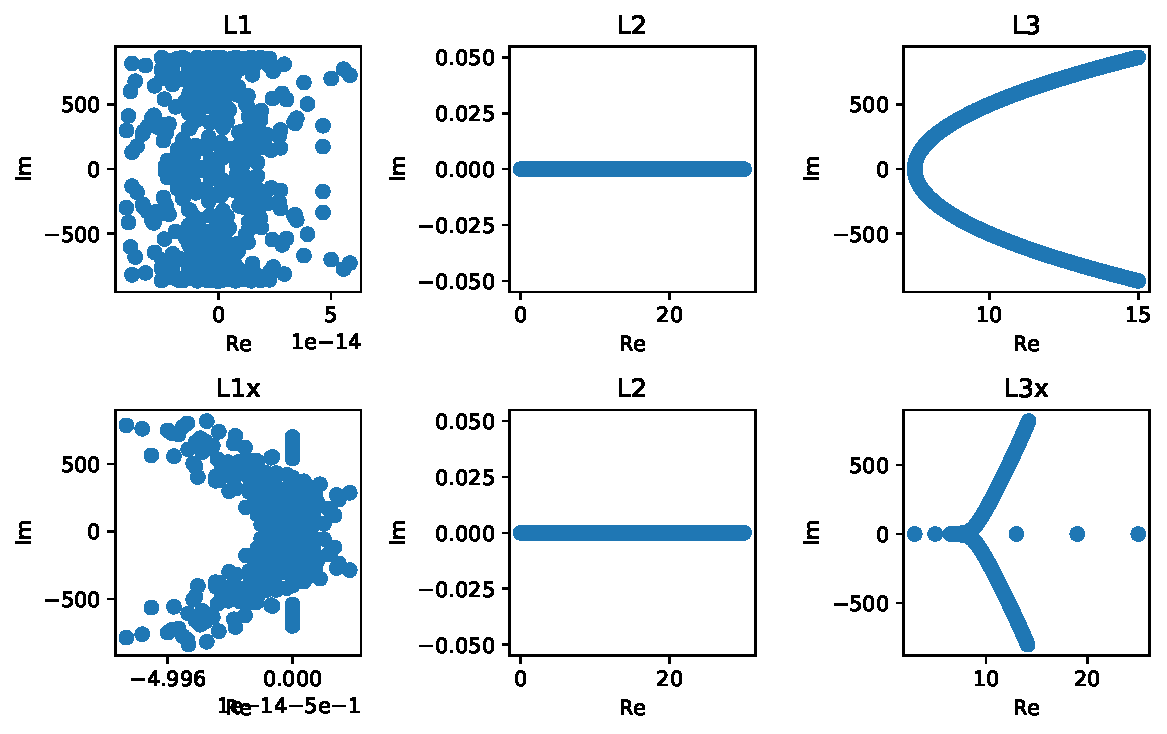
\includegraphics[width=0.8\textwidth]{eigs.pdf}
        \caption{Eigenvalues for the operators $L_1$, $L_2$, and $L_3$ with homogeneous Dirichlet conditions. Computed with $N = 500$ first-order Lagrange elements.\label{fig:eigenvalues}}
    \end{figure}
\end{solution}

\begin{exercise}{6.1}\label{ex:6.1}
    Show that the conditions in \cref{eq:6.15,eq:6.16,eq:6.17} are satisfied for $V_h = H^1_0$ and $Q_h = L^2$.
\end{exercise}

\begin{solution}{6.1}
    For this exercise we are considering Stokes problem, wherein we want to find $u_h \in V_h$ and $p_h \in Q_h$ such that
    \begin{equation}
        \begin{split}
            a(u_h, v_h) + b(p_h, v_h) &= f(v_h), \quad \forall v_h \in V_h, \\
            b(q_h, u_h) &= 0, \quad \forall q_h \in Q_h,
        \end{split}
    \end{equation}
    where
    \begin{equation}
        \begin{split}
            a(u, v) &= \int_{\Omega} \nabla u : \nabla v \diff x, \\
            b(p, v) &= \int_{\Omega} p \, \nabla \cdot v \diff x, \\
            f(v) &= \int_{\Omega} f \, v \diff x + \int_{\Omega_N} h \, v \diff s.
        \end{split}
    \end{equation}
    The conditions to show are then
    \begin{align}
        \text{\small Boundedness of $a$:}
        && \quad a(u_h, v_h) &\leq C_1 \norm{u_h}_{V_h} \norm{v_h}_{V_h},
        & \forall u_h, v_h \in V_h,
        \tag{6.15} \label{eq:6.15}
        \\
        \text{\small Boundedness of $b$:}
        && \quad b(q_h, u_h) &\leq C_2 \norm{q_h}_{Q_h} \norm{u_h}_{V_h},
        & \forall u_h \in V_h, q_h \in Q_h,
        \tag{6.16} \label{eq:6.16}
        \\
        \text{\small Coercivity of $a$:}
        && \quad a(u_h, u_h) &\geq C_3 \norm{u_h}_{V_h}^2,
        & \forall u_h \in Z_h,
        \tag{6.17} \label{eq:6.17}
    \end{align}
    where $Z_h = \{ u_h \in V_h \mid b(u_h, q_h) = 0, \, \forall q_h \in Q_h \}$.

    For \cref{eq:6.15}, we have
    \begin{equation}
        a(u_h, v_h) = \int_{\Omega} \nabla u_h : \nabla v_h \diff x,
    \end{equation}
    which by the Cauchy-Schwarz inequality is bounded by
    \begin{equation}
        a(u_h, v_h) \leq \norm{\nabla u_h}_{L^2} \norm{\nabla v_h}_{L^2} = \abs{u_h}_{H^1} \abs{v_h}_{H^1}.
    \end{equation}
    As we have previously shown that the $H^1$ semi-norm is equivalent to the $H^1$ norm, \cref{eq:6.15} is satisfied.

    For \cref{eq:6.16}, we have
    \begin{equation}
        b(q_h, u_h) = \int_{\Omega} q_h \, \nabla \cdot u_h \diff x,
    \end{equation}
    which by the Cauchy-Schwarz inequality is bounded by
    \begin{equation}
        b(q_h, u_h) \leq \norm{q_h}_{L^2} \norm{\nabla \cdot u_h}_{L^2}.
    \end{equation}
    We already have $\norm{q_h}_{L^2}$ as desired, and we now need to relate $\norm{\nabla \cdot u_h}_{L^2}$ to $\norm{\nabla u_h}_{L^2}$.
    We have
    \begin{align*}
        \abs{\nabla \cdot u(x)}^2
        &= \abs*{\sum_{i = 0}^{d} \frac{\partial u_i}{\partial x_i}(x)}^2
        \leq \left(
            \sum_{i = 0}^{d} 1
        \right) \left(
            \sum_{i = 0}^{d} \left( \frac{\partial u_i}{\partial x_i}(x) \right)^2
        \right)
        = d \sum_{i = 0}^{d} \left( \frac{\partial u_i}{\partial x_i}(x) \right)^2.
    \end{align*}
    Therefore,
    \begin{align*}
        \norm{\nabla \cdot u_h}_{L^2}^2
        &= \int_{\Omega} \abs{\nabla \cdot u_h}^2 \diff x
        \leq d \int_{\Omega} \sum_{i = 0}^{d} \left(
            \frac{\partial u_i}{\partial x_i}
        \right)^2 \diff x \\
        &\leq d \int_{\Omega} \sum_{i = 0}^{d} \sum_{j = 0}^{d} \left(
            \frac{\partial u_i}{\partial x_j}
        \right)^2 \diff x
        = d \int_{\Omega} \abs{\nabla u_h}^2 \diff x \\
        &= d \norm{\nabla u_h}_{L^2}^2.
    \end{align*}
    Using this, we have
    \begin{equation}
        b(q_h, u_h) \leq \sqrt{d} \norm{q_h}_{L^2} \norm{\nabla u_h}_{L^2},
    \end{equation}
    and as such \cref{eq:6.16} is satisfied.

    For \cref{eq:6.17}, we have
    \begin{equation}
        a(u_h, u_h)
        = \int_{\Omega} \nabla u_h : \nabla u_h \diff x
        = \norm{\nabla u_h}_{L^2}^2 = \abs{u_h}_{H^1}^2.
    \end{equation}
    As we have previously shown that the $H^1$ semi-norm is equivalent to the $H^1$ norm, \cref{eq:6.17} is satisfied.

    We have thus shown that the conditions in \cref{eq:6.15,eq:6.16,eq:6.17} are satisfied for $V_h = H^1_0$ and $Q_h = L^2$.
\end{solution}

\begin{exercise}{6.2}
    Show that the conditions in \cref{eq:6.15,eq:6.16,eq:6.17} are satisfied for Taylor--Hood and Mini discretizations. % chktex 8
    (Note that Crouzeix--Raviart is non-conforming so it is more difficult to prove these conditions for this case.) % chktex 8
\end{exercise}

\begin{solution}{6.2}
    The Taylor--Hood elements are defined by the basis functions % chktex 8
    \begin{equation}
        \begin{split}
            u &: N_i = a_i + b_i x + c_i y + d_i x y + e_i x^2 + f_i y^2, \\
            p &: L_i = k_i + l_i x + m_i y,
        \end{split}
    \end{equation}
    under the condition that $N_i$ is continuous across element boundaries.
    As such, we have that $u_h \in V_h \subset H^1_0$ and $p_h \in Q_h \subset L^2$ for the Taylor--Hood elements. % chktex 8
    They therefore satisfy the conditions in \cref{eq:6.15,eq:6.16,eq:6.17}, as shown in \cref{ex:6.1}.

    The Mini elements are, as far as I understand, defined by the basis functions
    \begin{equation}
        \begin{split}
            u &: N_i = a_i + b_i x + c_i y + d_i xy(1 - x - y), \\
            p &: L_i = k_i + l_i x + m_i y,
        \end{split}
    \end{equation}
    and we now need to show that $u_h \in V_h \subset H^1_0$.
    % With a slight abuse of notation, we have
    % \begin{align*}
    %     \nabla \cdot N_i &=
    %     \nabla \cdot (a_i + b_i x + c_i y + d_i xy - d_i x^2 y - d_i x y^2) \\
    %     &= b_i + c_i - d_i x^2 - 4d_i xy - d_i y^2 \\
    %     &= b_i + c_i - d_i (x^2 + 4xy + y^2).
    % \end{align*}
    % Presumably, we have that $V_h \subset H^1_0$, however I don't understand Fortin's trick.
    Notice that along each
\end{solution}

\begin{exercise}{6.6}
    In the previous problem the solution was a second order polynomial in the velocity and first order in the pressure.
    We may therefore obtain the exact solution and it is therefore difficult to check order of convergence for higher order methods with this solution.
    In this exercise you should therefore implement the problem
    \begin{align*}
        u &= (\sin(\pi y), \cos(\pi x)),
        & p &= \sin(2 \pi x),
        & f &= -\Delta u - \nabla p.
    \end{align*}
    Test whether the approximation is of the expected order for $P_4$--$P_3$, $P_4$--$P_2$, $P_3$--$P_2$, and $P_3$--$P_1$.
\end{exercise}

\begin{solution}{6.6}
    We begin by describing the weak formulation for Stokes problem, namely to find $u \in H_{D,0}^{1}$ and $p \in L^{2}$ such that
    \begin{align*}
        a(u, v) + b(p, v) &= f(v), & v &\in H_{D,0}^{1} \\
        b(q, u) &= 0, & q &\in L^{2},
    \end{align*}
    where
    \begin{align*}
        a(u, v) &= \int_{\Omega} \nabla u : \nabla v \, \diff x, \\
        b(p, v) &= \int_\Omega p \nabla \cdot v \, \diff x, \\
        f(v) &= \int_{\Omega} f \, v \, \diff x + \int_{\partial\Omega_N} h \, v \, \diff s.
    \end{align*}
    As far as I understand, we have for this problem $h = 0$, removing the Neumann boundary term.
    For the dirichlet term, we prescribe
    \begin{equation*}
        u = (\sin(\pi y), \cos(\pi x)) \quad \text{on } \partial\Omega_D,
    \end{equation*}
    where $\partial\Omega_D$ consists of the top, bottom and left boundaries.

    The solver is implemented in \texttt{stokes.py}\footnote{Add link to file on GitHub}, and the results are shown in \cref{fig:convergence}.
    The expected order of convergence rates is found through
    \begin{equation*}
        \norm{u - h_h}_1 + \norm{p - p_h} \leq C h^k \norm{u}_{k+1} + D h^{\ell + 1} \norm{p}_{\ell + 1},
    \end{equation*}
    where $k$ and $\ell$ are the polynomial degree of the velocity and pressure respectively.
    With the different elements, we would therefore expect convergence rates of
    \begin{align*}
        (P_4\text{--}P_3) &&  h^4 \norm{u}_{5} + D h^{4} \norm{p}_{4} &= h^4 (\norm{u}_{5} + D \norm{p}_{4}) \\
        (P_4\text{--}P_2) &&  h^4 \norm{u}_{5} + D h^{3} \norm{p}_{3} &= h^3 (h \norm{u}_{5} + D \norm{p}_{3}) \\
        (P_3\text{--}P_2) &&  h^3 \norm{u}_{4} + D h^{3} \norm{p}_{3} &= h^3 (\norm{u}_{4} + D \norm{p}_{3}) \\
        (P_3\text{--}P_1) &&  h^3 \norm{u}_{4} + D h^{2} \norm{p}_{2} &= h^2 (h \norm{u}_{3} + D \norm{p}_{2})
    \end{align*}
    As we see numerically in \cref{fig:convergence}, we get convergence of order 4, 3, 3, and 2 for the $P_4$--$P_3$, $P_4$--$P_2$, $P_3$--$P_2$, and $P_3$--$P_1$ elements, respectively, which aligns with our expectations.

    \begin{figure}[htbp]
        \centering
        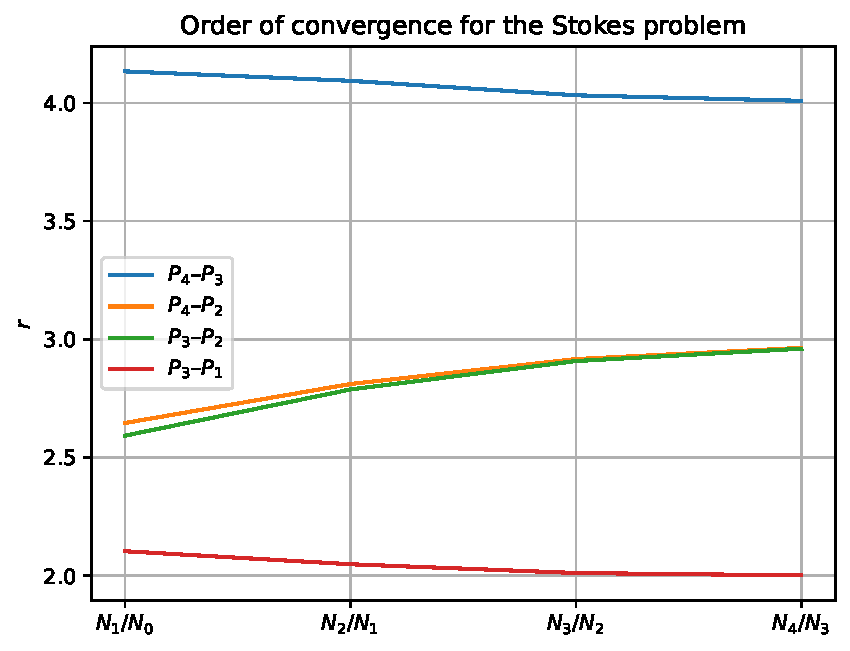
\includegraphics[
            width=0.8\textwidth,
            keepaspectratio,
        ]{stokes_convergence.pdf}
        \caption{Convergence of the $P_4$--$P_3$, $P_4$--$P_2$, $P_3$--$P_2$, and $P_3$--$P_1$ elements for the Stokes problem with the exact solution $u = (\sin(\pi y), \cos(\pi x))$ and $p = \sin(2 \pi x)$. Computed with $N = 4, 8, 16, 32, 64$.\label{fig:convergence}}
    \end{figure}
\end{solution}